% Copyright © 2013 Martin Ueding <dev@martin-ueding.de>
%
% Copyright © 2012-2013 Martin Ueding <dev@martin-ueding.de>

% This is my general purpose LaTeX header file for writing German documents.
% Ideally, you include this using a simple ``% Copyright © 2012-2013 Martin Ueding <dev@martin-ueding.de>

% This is my general purpose LaTeX header file for writing German documents.
% Ideally, you include this using a simple ``% Copyright © 2012-2013 Martin Ueding <dev@martin-ueding.de>

% This is my general purpose LaTeX header file for writing German documents.
% Ideally, you include this using a simple ``\input{header.tex}`` in your main
% document and start with ``\title`` and ``\begin{document}`` afterwards.

% If you need to add additional packages, I recommend not doing this in this
% file, but in your main document. That way, you can just drop in a new
% ``header.tex`` and get all the new commands without having to merge manually.

% Since this file encorporates a CC-BY-SA fragment, this whole files is
% licensed under the CC-BY-SA license.

\documentclass[11pt, ngerman, fleqn, DIV=15, headinclude]{scrartcl}

\usepackage{graphicx}

% Environment to quote the problem. Currently, this is just a new name for the
% quote environment.
\newenvironment{problem}{\begin{quote}}{\end{quote}}

%%%%%%%%%%%%%%%%%%%%%%%%%%%%%%%%%%%%%%%%%%%%%%%%%%%%%%%%%%%%%%%%%%%%%%%%%%%%%%%
%                                Locale, date                                 %
%%%%%%%%%%%%%%%%%%%%%%%%%%%%%%%%%%%%%%%%%%%%%%%%%%%%%%%%%%%%%%%%%%%%%%%%%%%%%%%

\usepackage{babel}
\usepackage[iso]{isodate}

%%%%%%%%%%%%%%%%%%%%%%%%%%%%%%%%%%%%%%%%%%%%%%%%%%%%%%%%%%%%%%%%%%%%%%%%%%%%%%%
%                          Margins and other spacing                          %
%%%%%%%%%%%%%%%%%%%%%%%%%%%%%%%%%%%%%%%%%%%%%%%%%%%%%%%%%%%%%%%%%%%%%%%%%%%%%%%

\usepackage[parfill]{parskip}
\usepackage{setspace}
\usepackage[activate]{microtype}

\setlength{\columnsep}{2cm}

%%%%%%%%%%%%%%%%%%%%%%%%%%%%%%%%%%%%%%%%%%%%%%%%%%%%%%%%%%%%%%%%%%%%%%%%%%%%%%%
%                                    Color                                    %
%%%%%%%%%%%%%%%%%%%%%%%%%%%%%%%%%%%%%%%%%%%%%%%%%%%%%%%%%%%%%%%%%%%%%%%%%%%%%%%

\usepackage[usenames, dvipsnames]{xcolor}

\colorlet{darkred}{red!70!black}
\colorlet{darkblue}{blue!70!black}
\colorlet{darkgreen}{green!40!black}

%%%%%%%%%%%%%%%%%%%%%%%%%%%%%%%%%%%%%%%%%%%%%%%%%%%%%%%%%%%%%%%%%%%%%%%%%%%%%%%
%                         Font and font like settings                         %
%%%%%%%%%%%%%%%%%%%%%%%%%%%%%%%%%%%%%%%%%%%%%%%%%%%%%%%%%%%%%%%%%%%%%%%%%%%%%%%

% This replaces all fonts with Bitstream Charter, Bitstream Vera Sans and
% Bitstream Vera Mono. Math will be rendered in Charter.
\usepackage[charter, greekuppercase=italicized]{mathdesign}
\usepackage{beramono}
\usepackage{berasans}

% Bold, sans-serif tensors. This fragment is taken from “egreg” from
% http://tex.stackexchange.com/a/82747/8945 and licensed under `CC-BY-SA
% <https://creativecommons.org/licenses/by-sa/3.0/>`_.
\usepackage{bm}
\DeclareMathAlphabet{\mathsfit}{\encodingdefault}{\sfdefault}{m}{sl}
\SetMathAlphabet{\mathsfit}{bold}{\encodingdefault}{\sfdefault}{bx}{sl}
\newcommand{\tens}[1]{\bm{\mathsfit{#1}}}

% Bold vectors.
\renewcommand{\vec}[1]{\boldsymbol{#1}}

%%%%%%%%%%%%%%%%%%%%%%%%%%%%%%%%%%%%%%%%%%%%%%%%%%%%%%%%%%%%%%%%%%%%%%%%%%%%%%%
%                               Input encoding                                %
%%%%%%%%%%%%%%%%%%%%%%%%%%%%%%%%%%%%%%%%%%%%%%%%%%%%%%%%%%%%%%%%%%%%%%%%%%%%%%%

\usepackage[T1]{fontenc}
\usepackage[utf8]{inputenc}

%%%%%%%%%%%%%%%%%%%%%%%%%%%%%%%%%%%%%%%%%%%%%%%%%%%%%%%%%%%%%%%%%%%%%%%%%%%%%%%
%                         Hyperrefs and PDF metadata                          %
%%%%%%%%%%%%%%%%%%%%%%%%%%%%%%%%%%%%%%%%%%%%%%%%%%%%%%%%%%%%%%%%%%%%%%%%%%%%%%%

\usepackage{hyperref}
\usepackage{lastpage}

% This sets the author in the properties of the PDF as well. If you want to
% change it, just override it with another ``\hypersetup`` call.
\hypersetup{
	breaklinks=false,
	citecolor=darkgreen,
	colorlinks=true,
	linkcolor=darkblue,
	menucolor=black,
	pdfauthor={Martin Ueding},
	urlcolor=darkblue,
}

%%%%%%%%%%%%%%%%%%%%%%%%%%%%%%%%%%%%%%%%%%%%%%%%%%%%%%%%%%%%%%%%%%%%%%%%%%%%%%%
%                               Math Operators                                %
%%%%%%%%%%%%%%%%%%%%%%%%%%%%%%%%%%%%%%%%%%%%%%%%%%%%%%%%%%%%%%%%%%%%%%%%%%%%%%%

% AMS environments like ``align`` and theorems like ``proof``.
\usepackage{amsmath}
\usepackage{amsthm}

% Common math constructs like partial derivatives.
\usepackage{commath}

% Physical units.
\usepackage[output-decimal-marker={,}]{siunitx}

% Word like operators.
\DeclareMathOperator{\acosh}{arcosh}
\DeclareMathOperator{\arcosh}{arcosh}
\DeclareMathOperator{\arcsinh}{arsinh}
\DeclareMathOperator{\arsinh}{arsinh}
\DeclareMathOperator{\asinh}{arsinh}
\DeclareMathOperator{\card}{card}
\DeclareMathOperator{\csch}{cshs}
\DeclareMathOperator{\diam}{diam}
\DeclareMathOperator{\sech}{sech}
\renewcommand{\Im}{\mathop{{}\mathrm{Im}}\nolimits}
\renewcommand{\Re}{\mathop{{}\mathrm{Re}}\nolimits}

% Fourier transform.
\DeclareMathOperator{\fourier}{\ensuremath{\mathcal{F}}}

% Roman versions of “e” and “i” to serve as Euler's number and the imaginary
% constant.
\newcommand{\ee}{\eup}
\newcommand{\eup}{\mathrm e}
\newcommand{\ii}{\iup}
\newcommand{\iup}{\mathrm i}

% Symbols for the various mathematical fields (natural numbers, integers,
% rational numbers, real numbers, complex numbers).
\newcommand{\C}{\ensuremath{\mathbb C}}
\newcommand{\N}{\ensuremath{\mathbb N}}
\newcommand{\Q}{\ensuremath{\mathbb Q}}
\newcommand{\R}{\ensuremath{\mathbb R}}
\newcommand{\Z}{\ensuremath{\mathbb Z}}

% Shape like operators.
\DeclareMathOperator{\dalambert}{\Box}
\DeclareMathOperator{\laplace}{\bigtriangleup}
\newcommand{\curl}{\vnabla \times}
\newcommand{\divergence}[1]{\inner{\vnabla}{#1}}
\newcommand{\vnabla}{\vec \nabla}

\newcommand{\half}{\frac 12}

% Unit vector (German „Einheitsvektor“).
\newcommand{\ev}{\hat{\vec e}}

% Scientific notation for large numbers.
\newcommand{\e}[1]{\cdot 10^{#1}}

% Mathematician's notation for the inner (scalar, dot) product.
\newcommand{\bracket}[1]{\left\langle #1 \right\rangle}
\newcommand{\inner}[2]{\bracket{#1, #2}}

% Placeholders.
\newcommand{\emesswert}{\del{\messwert \pm \messwert}}
\newcommand{\fehlt}{\textcolor{darkred}{Hier fehlen noch Inhalte.}}
\newcommand{\messwert}{\textcolor{blue}{\square}}
\newcommand{\punkte}{\phantom{xxxxx}}
\newcommand{\punktevon}[1]{\begin{flushright}/ #1\end{flushright}}

% Separator for equations on a single line.
\newcommand{\eqnsep}{,\quad}

% Quantum Mechanics
\newcommand{\braket}[2]{\left\langle #1 \left. \vphantom{#1 #2} \right| #2 \right\rangle}
\newcommand{\braopket}[3]{\left\langle #1 \left. \vphantom{#1 #2 #3} \right| #2 \left. \vphantom{#1 #2 #3} \right| #3 \right\rangle}
\newcommand{\bra}[1]{\left\langle #1 \right|}
\newcommand{\ketbra}[2]{\left| #1 \vphantom{#2} \right\rangle \left\langle #2  \vphantom{#1} \right|}
\newcommand{\ket}[1]{\left| #1 \right\rangle}

%%%%%%%%%%%%%%%%%%%%%%%%%%%%%%%%%%%%%%%%%%%%%%%%%%%%%%%%%%%%%%%%%%%%%%%%%%%%%%%
%                                  Headings                                   %
%%%%%%%%%%%%%%%%%%%%%%%%%%%%%%%%%%%%%%%%%%%%%%%%%%%%%%%%%%%%%%%%%%%%%%%%%%%%%%%

% This will set fancy headings to the top of the page. The page number will be
% accompanied by the total number of pages. That way, you will know if any page
% is missing.
%
% If you do not want this for your document, you can just use
% ``\pagestyle{plain}``.

\usepackage{scrpage2}

\pagestyle{scrheadings}
\automark{section}
\cfoot{\footnotesize{Seite \thepage\ / \pageref{LastPage}}}
\chead{}
\ihead{}
\ohead{\rightmark}
\setheadsepline{.4pt}

%%%%%%%%%%%%%%%%%%%%%%%%%%%%%%%%%%%%%%%%%%%%%%%%%%%%%%%%%%%%%%%%%%%%%%%%%%%%%%%
%                            Bibliography (BibTeX)                            %
%%%%%%%%%%%%%%%%%%%%%%%%%%%%%%%%%%%%%%%%%%%%%%%%%%%%%%%%%%%%%%%%%%%%%%%%%%%%%%%

\newcommand{\bibliographyfile}{../../zentrale_BibTeX/Central}
\bibliographystyle{apalike2}

%%%%%%%%%%%%%%%%%%%%%%%%%%%%%%%%%%%%%%%%%%%%%%%%%%%%%%%%%%%%%%%%%%%%%%%%%%%%%%%
%                                Abbreviations                                %
%%%%%%%%%%%%%%%%%%%%%%%%%%%%%%%%%%%%%%%%%%%%%%%%%%%%%%%%%%%%%%%%%%%%%%%%%%%%%%%

\newcommand{\dhabk}{\mbox{d.\,h.}}

%%%%%%%%%%%%%%%%%%%%%%%%%%%%%%%%%%%%%%%%%%%%%%%%%%%%%%%%%%%%%%%%%%%%%%%%%%%%%%%
%                                  Licences                                   %
%%%%%%%%%%%%%%%%%%%%%%%%%%%%%%%%%%%%%%%%%%%%%%%%%%%%%%%%%%%%%%%%%%%%%%%%%%%%%%%

\usepackage{ccicons}

\newcommand{\ccbysadetext}{%
	\begin{small}
		Dieses Werk bzw. Inhalt steht unter einer
		\href{http://creativecommons.org/licenses/by-sa/3.0/deed.de}{%
			Creative Commons Namensnennung - Weitergabe unter gleichen
		Bedingungen 3.0 Unported Lizenz}.
	\end{small}
}

\newcommand{\ccbysadetitle}{%
	Lizenz: \href{http://creativecommons.org/licenses/by-sa/3.0/deed.de}
	{CC-BY-SA 3.0 \ccbysa}
}
`` in your main
% document and start with ``\title`` and ``\begin{document}`` afterwards.

% If you need to add additional packages, I recommend not doing this in this
% file, but in your main document. That way, you can just drop in a new
% ``header.tex`` and get all the new commands without having to merge manually.

% Since this file encorporates a CC-BY-SA fragment, this whole files is
% licensed under the CC-BY-SA license.

\documentclass[11pt, ngerman, fleqn, DIV=15, headinclude]{scrartcl}

\usepackage{graphicx}

% Environment to quote the problem. Currently, this is just a new name for the
% quote environment.
\newenvironment{problem}{\begin{quote}}{\end{quote}}

%%%%%%%%%%%%%%%%%%%%%%%%%%%%%%%%%%%%%%%%%%%%%%%%%%%%%%%%%%%%%%%%%%%%%%%%%%%%%%%
%                                Locale, date                                 %
%%%%%%%%%%%%%%%%%%%%%%%%%%%%%%%%%%%%%%%%%%%%%%%%%%%%%%%%%%%%%%%%%%%%%%%%%%%%%%%

\usepackage{babel}
\usepackage[iso]{isodate}

%%%%%%%%%%%%%%%%%%%%%%%%%%%%%%%%%%%%%%%%%%%%%%%%%%%%%%%%%%%%%%%%%%%%%%%%%%%%%%%
%                          Margins and other spacing                          %
%%%%%%%%%%%%%%%%%%%%%%%%%%%%%%%%%%%%%%%%%%%%%%%%%%%%%%%%%%%%%%%%%%%%%%%%%%%%%%%

\usepackage[parfill]{parskip}
\usepackage{setspace}
\usepackage[activate]{microtype}

\setlength{\columnsep}{2cm}

%%%%%%%%%%%%%%%%%%%%%%%%%%%%%%%%%%%%%%%%%%%%%%%%%%%%%%%%%%%%%%%%%%%%%%%%%%%%%%%
%                                    Color                                    %
%%%%%%%%%%%%%%%%%%%%%%%%%%%%%%%%%%%%%%%%%%%%%%%%%%%%%%%%%%%%%%%%%%%%%%%%%%%%%%%

\usepackage[usenames, dvipsnames]{xcolor}

\colorlet{darkred}{red!70!black}
\colorlet{darkblue}{blue!70!black}
\colorlet{darkgreen}{green!40!black}

%%%%%%%%%%%%%%%%%%%%%%%%%%%%%%%%%%%%%%%%%%%%%%%%%%%%%%%%%%%%%%%%%%%%%%%%%%%%%%%
%                         Font and font like settings                         %
%%%%%%%%%%%%%%%%%%%%%%%%%%%%%%%%%%%%%%%%%%%%%%%%%%%%%%%%%%%%%%%%%%%%%%%%%%%%%%%

% This replaces all fonts with Bitstream Charter, Bitstream Vera Sans and
% Bitstream Vera Mono. Math will be rendered in Charter.
\usepackage[charter, greekuppercase=italicized]{mathdesign}
\usepackage{beramono}
\usepackage{berasans}

% Bold, sans-serif tensors. This fragment is taken from “egreg” from
% http://tex.stackexchange.com/a/82747/8945 and licensed under `CC-BY-SA
% <https://creativecommons.org/licenses/by-sa/3.0/>`_.
\usepackage{bm}
\DeclareMathAlphabet{\mathsfit}{\encodingdefault}{\sfdefault}{m}{sl}
\SetMathAlphabet{\mathsfit}{bold}{\encodingdefault}{\sfdefault}{bx}{sl}
\newcommand{\tens}[1]{\bm{\mathsfit{#1}}}

% Bold vectors.
\renewcommand{\vec}[1]{\boldsymbol{#1}}

%%%%%%%%%%%%%%%%%%%%%%%%%%%%%%%%%%%%%%%%%%%%%%%%%%%%%%%%%%%%%%%%%%%%%%%%%%%%%%%
%                               Input encoding                                %
%%%%%%%%%%%%%%%%%%%%%%%%%%%%%%%%%%%%%%%%%%%%%%%%%%%%%%%%%%%%%%%%%%%%%%%%%%%%%%%

\usepackage[T1]{fontenc}
\usepackage[utf8]{inputenc}

%%%%%%%%%%%%%%%%%%%%%%%%%%%%%%%%%%%%%%%%%%%%%%%%%%%%%%%%%%%%%%%%%%%%%%%%%%%%%%%
%                         Hyperrefs and PDF metadata                          %
%%%%%%%%%%%%%%%%%%%%%%%%%%%%%%%%%%%%%%%%%%%%%%%%%%%%%%%%%%%%%%%%%%%%%%%%%%%%%%%

\usepackage{hyperref}
\usepackage{lastpage}

% This sets the author in the properties of the PDF as well. If you want to
% change it, just override it with another ``\hypersetup`` call.
\hypersetup{
	breaklinks=false,
	citecolor=darkgreen,
	colorlinks=true,
	linkcolor=darkblue,
	menucolor=black,
	pdfauthor={Martin Ueding},
	urlcolor=darkblue,
}

%%%%%%%%%%%%%%%%%%%%%%%%%%%%%%%%%%%%%%%%%%%%%%%%%%%%%%%%%%%%%%%%%%%%%%%%%%%%%%%
%                               Math Operators                                %
%%%%%%%%%%%%%%%%%%%%%%%%%%%%%%%%%%%%%%%%%%%%%%%%%%%%%%%%%%%%%%%%%%%%%%%%%%%%%%%

% AMS environments like ``align`` and theorems like ``proof``.
\usepackage{amsmath}
\usepackage{amsthm}

% Common math constructs like partial derivatives.
\usepackage{commath}

% Physical units.
\usepackage[output-decimal-marker={,}]{siunitx}

% Word like operators.
\DeclareMathOperator{\acosh}{arcosh}
\DeclareMathOperator{\arcosh}{arcosh}
\DeclareMathOperator{\arcsinh}{arsinh}
\DeclareMathOperator{\arsinh}{arsinh}
\DeclareMathOperator{\asinh}{arsinh}
\DeclareMathOperator{\card}{card}
\DeclareMathOperator{\csch}{cshs}
\DeclareMathOperator{\diam}{diam}
\DeclareMathOperator{\sech}{sech}
\renewcommand{\Im}{\mathop{{}\mathrm{Im}}\nolimits}
\renewcommand{\Re}{\mathop{{}\mathrm{Re}}\nolimits}

% Fourier transform.
\DeclareMathOperator{\fourier}{\ensuremath{\mathcal{F}}}

% Roman versions of “e” and “i” to serve as Euler's number and the imaginary
% constant.
\newcommand{\ee}{\eup}
\newcommand{\eup}{\mathrm e}
\newcommand{\ii}{\iup}
\newcommand{\iup}{\mathrm i}

% Symbols for the various mathematical fields (natural numbers, integers,
% rational numbers, real numbers, complex numbers).
\newcommand{\C}{\ensuremath{\mathbb C}}
\newcommand{\N}{\ensuremath{\mathbb N}}
\newcommand{\Q}{\ensuremath{\mathbb Q}}
\newcommand{\R}{\ensuremath{\mathbb R}}
\newcommand{\Z}{\ensuremath{\mathbb Z}}

% Shape like operators.
\DeclareMathOperator{\dalambert}{\Box}
\DeclareMathOperator{\laplace}{\bigtriangleup}
\newcommand{\curl}{\vnabla \times}
\newcommand{\divergence}[1]{\inner{\vnabla}{#1}}
\newcommand{\vnabla}{\vec \nabla}

\newcommand{\half}{\frac 12}

% Unit vector (German „Einheitsvektor“).
\newcommand{\ev}{\hat{\vec e}}

% Scientific notation for large numbers.
\newcommand{\e}[1]{\cdot 10^{#1}}

% Mathematician's notation for the inner (scalar, dot) product.
\newcommand{\bracket}[1]{\left\langle #1 \right\rangle}
\newcommand{\inner}[2]{\bracket{#1, #2}}

% Placeholders.
\newcommand{\emesswert}{\del{\messwert \pm \messwert}}
\newcommand{\fehlt}{\textcolor{darkred}{Hier fehlen noch Inhalte.}}
\newcommand{\messwert}{\textcolor{blue}{\square}}
\newcommand{\punkte}{\phantom{xxxxx}}
\newcommand{\punktevon}[1]{\begin{flushright}/ #1\end{flushright}}

% Separator for equations on a single line.
\newcommand{\eqnsep}{,\quad}

% Quantum Mechanics
\newcommand{\braket}[2]{\left\langle #1 \left. \vphantom{#1 #2} \right| #2 \right\rangle}
\newcommand{\braopket}[3]{\left\langle #1 \left. \vphantom{#1 #2 #3} \right| #2 \left. \vphantom{#1 #2 #3} \right| #3 \right\rangle}
\newcommand{\bra}[1]{\left\langle #1 \right|}
\newcommand{\ketbra}[2]{\left| #1 \vphantom{#2} \right\rangle \left\langle #2  \vphantom{#1} \right|}
\newcommand{\ket}[1]{\left| #1 \right\rangle}

%%%%%%%%%%%%%%%%%%%%%%%%%%%%%%%%%%%%%%%%%%%%%%%%%%%%%%%%%%%%%%%%%%%%%%%%%%%%%%%
%                                  Headings                                   %
%%%%%%%%%%%%%%%%%%%%%%%%%%%%%%%%%%%%%%%%%%%%%%%%%%%%%%%%%%%%%%%%%%%%%%%%%%%%%%%

% This will set fancy headings to the top of the page. The page number will be
% accompanied by the total number of pages. That way, you will know if any page
% is missing.
%
% If you do not want this for your document, you can just use
% ``\pagestyle{plain}``.

\usepackage{scrpage2}

\pagestyle{scrheadings}
\automark{section}
\cfoot{\footnotesize{Seite \thepage\ / \pageref{LastPage}}}
\chead{}
\ihead{}
\ohead{\rightmark}
\setheadsepline{.4pt}

%%%%%%%%%%%%%%%%%%%%%%%%%%%%%%%%%%%%%%%%%%%%%%%%%%%%%%%%%%%%%%%%%%%%%%%%%%%%%%%
%                            Bibliography (BibTeX)                            %
%%%%%%%%%%%%%%%%%%%%%%%%%%%%%%%%%%%%%%%%%%%%%%%%%%%%%%%%%%%%%%%%%%%%%%%%%%%%%%%

\newcommand{\bibliographyfile}{../../zentrale_BibTeX/Central}
\bibliographystyle{apalike2}

%%%%%%%%%%%%%%%%%%%%%%%%%%%%%%%%%%%%%%%%%%%%%%%%%%%%%%%%%%%%%%%%%%%%%%%%%%%%%%%
%                                Abbreviations                                %
%%%%%%%%%%%%%%%%%%%%%%%%%%%%%%%%%%%%%%%%%%%%%%%%%%%%%%%%%%%%%%%%%%%%%%%%%%%%%%%

\newcommand{\dhabk}{\mbox{d.\,h.}}

%%%%%%%%%%%%%%%%%%%%%%%%%%%%%%%%%%%%%%%%%%%%%%%%%%%%%%%%%%%%%%%%%%%%%%%%%%%%%%%
%                                  Licences                                   %
%%%%%%%%%%%%%%%%%%%%%%%%%%%%%%%%%%%%%%%%%%%%%%%%%%%%%%%%%%%%%%%%%%%%%%%%%%%%%%%

\usepackage{ccicons}

\newcommand{\ccbysadetext}{%
	\begin{small}
		Dieses Werk bzw. Inhalt steht unter einer
		\href{http://creativecommons.org/licenses/by-sa/3.0/deed.de}{%
			Creative Commons Namensnennung - Weitergabe unter gleichen
		Bedingungen 3.0 Unported Lizenz}.
	\end{small}
}

\newcommand{\ccbysadetitle}{%
	Lizenz: \href{http://creativecommons.org/licenses/by-sa/3.0/deed.de}
	{CC-BY-SA 3.0 \ccbysa}
}
`` in your main
% document and start with ``\title`` and ``\begin{document}`` afterwards.

% If you need to add additional packages, I recommend not doing this in this
% file, but in your main document. That way, you can just drop in a new
% ``header.tex`` and get all the new commands without having to merge manually.

% Since this file encorporates a CC-BY-SA fragment, this whole files is
% licensed under the CC-BY-SA license.

\documentclass[11pt, ngerman, fleqn, DIV=15, headinclude]{scrartcl}

\usepackage{graphicx}

% Environment to quote the problem. Currently, this is just a new name for the
% quote environment.
\newenvironment{problem}{\begin{quote}}{\end{quote}}

%%%%%%%%%%%%%%%%%%%%%%%%%%%%%%%%%%%%%%%%%%%%%%%%%%%%%%%%%%%%%%%%%%%%%%%%%%%%%%%
%                                Locale, date                                 %
%%%%%%%%%%%%%%%%%%%%%%%%%%%%%%%%%%%%%%%%%%%%%%%%%%%%%%%%%%%%%%%%%%%%%%%%%%%%%%%

\usepackage{babel}
\usepackage[iso]{isodate}

%%%%%%%%%%%%%%%%%%%%%%%%%%%%%%%%%%%%%%%%%%%%%%%%%%%%%%%%%%%%%%%%%%%%%%%%%%%%%%%
%                          Margins and other spacing                          %
%%%%%%%%%%%%%%%%%%%%%%%%%%%%%%%%%%%%%%%%%%%%%%%%%%%%%%%%%%%%%%%%%%%%%%%%%%%%%%%

\usepackage[parfill]{parskip}
\usepackage{setspace}
\usepackage[activate]{microtype}

\setlength{\columnsep}{2cm}

%%%%%%%%%%%%%%%%%%%%%%%%%%%%%%%%%%%%%%%%%%%%%%%%%%%%%%%%%%%%%%%%%%%%%%%%%%%%%%%
%                                    Color                                    %
%%%%%%%%%%%%%%%%%%%%%%%%%%%%%%%%%%%%%%%%%%%%%%%%%%%%%%%%%%%%%%%%%%%%%%%%%%%%%%%

\usepackage[usenames, dvipsnames]{xcolor}

\colorlet{darkred}{red!70!black}
\colorlet{darkblue}{blue!70!black}
\colorlet{darkgreen}{green!40!black}

%%%%%%%%%%%%%%%%%%%%%%%%%%%%%%%%%%%%%%%%%%%%%%%%%%%%%%%%%%%%%%%%%%%%%%%%%%%%%%%
%                         Font and font like settings                         %
%%%%%%%%%%%%%%%%%%%%%%%%%%%%%%%%%%%%%%%%%%%%%%%%%%%%%%%%%%%%%%%%%%%%%%%%%%%%%%%

% This replaces all fonts with Bitstream Charter, Bitstream Vera Sans and
% Bitstream Vera Mono. Math will be rendered in Charter.
\usepackage[charter, greekuppercase=italicized]{mathdesign}
\usepackage{beramono}
\usepackage{berasans}

% Bold, sans-serif tensors. This fragment is taken from “egreg” from
% http://tex.stackexchange.com/a/82747/8945 and licensed under `CC-BY-SA
% <https://creativecommons.org/licenses/by-sa/3.0/>`_.
\usepackage{bm}
\DeclareMathAlphabet{\mathsfit}{\encodingdefault}{\sfdefault}{m}{sl}
\SetMathAlphabet{\mathsfit}{bold}{\encodingdefault}{\sfdefault}{bx}{sl}
\newcommand{\tens}[1]{\bm{\mathsfit{#1}}}

% Bold vectors.
\renewcommand{\vec}[1]{\boldsymbol{#1}}

%%%%%%%%%%%%%%%%%%%%%%%%%%%%%%%%%%%%%%%%%%%%%%%%%%%%%%%%%%%%%%%%%%%%%%%%%%%%%%%
%                               Input encoding                                %
%%%%%%%%%%%%%%%%%%%%%%%%%%%%%%%%%%%%%%%%%%%%%%%%%%%%%%%%%%%%%%%%%%%%%%%%%%%%%%%

\usepackage[T1]{fontenc}
\usepackage[utf8]{inputenc}

%%%%%%%%%%%%%%%%%%%%%%%%%%%%%%%%%%%%%%%%%%%%%%%%%%%%%%%%%%%%%%%%%%%%%%%%%%%%%%%
%                         Hyperrefs and PDF metadata                          %
%%%%%%%%%%%%%%%%%%%%%%%%%%%%%%%%%%%%%%%%%%%%%%%%%%%%%%%%%%%%%%%%%%%%%%%%%%%%%%%

\usepackage{hyperref}
\usepackage{lastpage}

% This sets the author in the properties of the PDF as well. If you want to
% change it, just override it with another ``\hypersetup`` call.
\hypersetup{
	breaklinks=false,
	citecolor=darkgreen,
	colorlinks=true,
	linkcolor=darkblue,
	menucolor=black,
	pdfauthor={Martin Ueding},
	urlcolor=darkblue,
}

%%%%%%%%%%%%%%%%%%%%%%%%%%%%%%%%%%%%%%%%%%%%%%%%%%%%%%%%%%%%%%%%%%%%%%%%%%%%%%%
%                               Math Operators                                %
%%%%%%%%%%%%%%%%%%%%%%%%%%%%%%%%%%%%%%%%%%%%%%%%%%%%%%%%%%%%%%%%%%%%%%%%%%%%%%%

% AMS environments like ``align`` and theorems like ``proof``.
\usepackage{amsmath}
\usepackage{amsthm}

% Common math constructs like partial derivatives.
\usepackage{commath}

% Physical units.
\usepackage[output-decimal-marker={,}]{siunitx}

% Word like operators.
\DeclareMathOperator{\acosh}{arcosh}
\DeclareMathOperator{\arcosh}{arcosh}
\DeclareMathOperator{\arcsinh}{arsinh}
\DeclareMathOperator{\arsinh}{arsinh}
\DeclareMathOperator{\asinh}{arsinh}
\DeclareMathOperator{\card}{card}
\DeclareMathOperator{\csch}{cshs}
\DeclareMathOperator{\diam}{diam}
\DeclareMathOperator{\sech}{sech}
\renewcommand{\Im}{\mathop{{}\mathrm{Im}}\nolimits}
\renewcommand{\Re}{\mathop{{}\mathrm{Re}}\nolimits}

% Fourier transform.
\DeclareMathOperator{\fourier}{\ensuremath{\mathcal{F}}}

% Roman versions of “e” and “i” to serve as Euler's number and the imaginary
% constant.
\newcommand{\ee}{\eup}
\newcommand{\eup}{\mathrm e}
\newcommand{\ii}{\iup}
\newcommand{\iup}{\mathrm i}

% Symbols for the various mathematical fields (natural numbers, integers,
% rational numbers, real numbers, complex numbers).
\newcommand{\C}{\ensuremath{\mathbb C}}
\newcommand{\N}{\ensuremath{\mathbb N}}
\newcommand{\Q}{\ensuremath{\mathbb Q}}
\newcommand{\R}{\ensuremath{\mathbb R}}
\newcommand{\Z}{\ensuremath{\mathbb Z}}

% Shape like operators.
\DeclareMathOperator{\dalambert}{\Box}
\DeclareMathOperator{\laplace}{\bigtriangleup}
\newcommand{\curl}{\vnabla \times}
\newcommand{\divergence}[1]{\inner{\vnabla}{#1}}
\newcommand{\vnabla}{\vec \nabla}

\newcommand{\half}{\frac 12}

% Unit vector (German „Einheitsvektor“).
\newcommand{\ev}{\hat{\vec e}}

% Scientific notation for large numbers.
\newcommand{\e}[1]{\cdot 10^{#1}}

% Mathematician's notation for the inner (scalar, dot) product.
\newcommand{\bracket}[1]{\left\langle #1 \right\rangle}
\newcommand{\inner}[2]{\bracket{#1, #2}}

% Placeholders.
\newcommand{\emesswert}{\del{\messwert \pm \messwert}}
\newcommand{\fehlt}{\textcolor{darkred}{Hier fehlen noch Inhalte.}}
\newcommand{\messwert}{\textcolor{blue}{\square}}
\newcommand{\punkte}{\phantom{xxxxx}}
\newcommand{\punktevon}[1]{\begin{flushright}/ #1\end{flushright}}

% Separator for equations on a single line.
\newcommand{\eqnsep}{,\quad}

% Quantum Mechanics
\newcommand{\braket}[2]{\left\langle #1 \left. \vphantom{#1 #2} \right| #2 \right\rangle}
\newcommand{\braopket}[3]{\left\langle #1 \left. \vphantom{#1 #2 #3} \right| #2 \left. \vphantom{#1 #2 #3} \right| #3 \right\rangle}
\newcommand{\bra}[1]{\left\langle #1 \right|}
\newcommand{\ketbra}[2]{\left| #1 \vphantom{#2} \right\rangle \left\langle #2  \vphantom{#1} \right|}
\newcommand{\ket}[1]{\left| #1 \right\rangle}

%%%%%%%%%%%%%%%%%%%%%%%%%%%%%%%%%%%%%%%%%%%%%%%%%%%%%%%%%%%%%%%%%%%%%%%%%%%%%%%
%                                  Headings                                   %
%%%%%%%%%%%%%%%%%%%%%%%%%%%%%%%%%%%%%%%%%%%%%%%%%%%%%%%%%%%%%%%%%%%%%%%%%%%%%%%

% This will set fancy headings to the top of the page. The page number will be
% accompanied by the total number of pages. That way, you will know if any page
% is missing.
%
% If you do not want this for your document, you can just use
% ``\pagestyle{plain}``.

\usepackage{scrpage2}

\pagestyle{scrheadings}
\automark{section}
\cfoot{\footnotesize{Seite \thepage\ / \pageref{LastPage}}}
\chead{}
\ihead{}
\ohead{\rightmark}
\setheadsepline{.4pt}

%%%%%%%%%%%%%%%%%%%%%%%%%%%%%%%%%%%%%%%%%%%%%%%%%%%%%%%%%%%%%%%%%%%%%%%%%%%%%%%
%                            Bibliography (BibTeX)                            %
%%%%%%%%%%%%%%%%%%%%%%%%%%%%%%%%%%%%%%%%%%%%%%%%%%%%%%%%%%%%%%%%%%%%%%%%%%%%%%%

\newcommand{\bibliographyfile}{../../zentrale_BibTeX/Central}
\bibliographystyle{apalike2}

%%%%%%%%%%%%%%%%%%%%%%%%%%%%%%%%%%%%%%%%%%%%%%%%%%%%%%%%%%%%%%%%%%%%%%%%%%%%%%%
%                                Abbreviations                                %
%%%%%%%%%%%%%%%%%%%%%%%%%%%%%%%%%%%%%%%%%%%%%%%%%%%%%%%%%%%%%%%%%%%%%%%%%%%%%%%

\newcommand{\dhabk}{\mbox{d.\,h.}}

%%%%%%%%%%%%%%%%%%%%%%%%%%%%%%%%%%%%%%%%%%%%%%%%%%%%%%%%%%%%%%%%%%%%%%%%%%%%%%%
%                                  Licences                                   %
%%%%%%%%%%%%%%%%%%%%%%%%%%%%%%%%%%%%%%%%%%%%%%%%%%%%%%%%%%%%%%%%%%%%%%%%%%%%%%%

\usepackage{ccicons}

\newcommand{\ccbysadetext}{%
	\begin{small}
		Dieses Werk bzw. Inhalt steht unter einer
		\href{http://creativecommons.org/licenses/by-sa/3.0/deed.de}{%
			Creative Commons Namensnennung - Weitergabe unter gleichen
		Bedingungen 3.0 Unported Lizenz}.
	\end{small}
}

\newcommand{\ccbysadetitle}{%
	Lizenz: \href{http://creativecommons.org/licenses/by-sa/3.0/deed.de}
	{CC-BY-SA 3.0 \ccbysa}
}


\usepackage{tikz}
\usetikzlibrary{calc}

\newcommand{\themodul}{physik411}
\newcommand{\thegruppe}{Gruppe 2 -- Florian Seidler}
\newcommand{\theuebung}{9}

\ifoot{\footnotesize{Martin Ueding}}
\ihead{\themodul{} -- Übung \theuebung}
\ofoot{\footnotesize{\thegruppe}}

\def\thesubsection{\thesection\alph{subsection}}

\title{\themodul{} -- Übung \theuebung}
\subtitle{\thegruppe}
\author{
	Martin Ueding \footnote{\href{mailto:mu@uni-bonn.de}{mu@uni-bonn.de}}
}

\hypersetup{
	pdftitle={\themodul {} - Übung \theuebung},
}

\begin{document}

\maketitle

\begin{center}
	\ccbysadetitle
\end{center}

\begin{table}[h]
	\centering
	\begin{tabular}{l*5{|c}}
		Aufgabe
		& \ref 1
		& \ref 2
		& \ref 3
		& \ref 4
		& $\sum$   \\
		\hline
		Punkte
		& \punkte / 7
		& \punkte / 18
		& \punkte / 14
		& \punkte / 10
		& \punkte / 49
	\end{tabular}
\end{table}

%%%%%%%%%%%%%%%%%%%%%%%%%%%%%%%%%%%%%%%%%%%%%%%%%%%%%%%%%%%%%%%%%%%%%%%%%%%%%%%
%                             Chemische Bindungen                             %
%%%%%%%%%%%%%%%%%%%%%%%%%%%%%%%%%%%%%%%%%%%%%%%%%%%%%%%%%%%%%%%%%%%%%%%%%%%%%%%

\section{Chemische Bindungen}
\label 1

\subsection{Art der Bindung}

Bei NaCl ist die Bindung eine ionische Bindung, da sich die Orbitale nicht
wirklich überlappen.

Beim Silizium sind die Elektronenwolken schon noch lokalisiert, es ist also
keine ionische Bindung. Da allerdings die Elektronen nicht delokalisiert sind,
sollte es sich um eine kovalente Bindung handeln. Silizium ist ein Halbleiter,
der im Grundzustand isoliert und wenig freie, delokalisierte Elektronen hat.

\subsection{(Un)gerichtete Bindung}

Beim NaCl handelt es sich wahrscheinlich um eine ungerichtete Bindung, da die
Ionen keine wirkliche Bindung miteinander eingeben, die Orbitale sind noch
einigermaßen rund, und nicht zu einer $\sigmaup$-Bindung zusammen. Zwar
überlappen sich die Orbitale ein wenig, haben aber keine wirkliche $\sigmaup$-
oder $\piup$-Bindung.

Beim Silizium ist die Bindung zwischen zwei Atomkernen zu erkennen, es handelt
sich um eine gerichtete Bindung.

\subsection{Bloch-Wellen}

In der Vorlesung von \date{2013-06-07} wurde der Realteil des Potentials
$u_k(r)$ gezeigt. Es hatte einige stark negative Peaks zwischen den Atomen, so
dass die Wahrscheinlichkeitsverteilung wahrscheinlich auch Spitzen hat. Jedoch
klingen delokalisierte Elektronen, die sich nahezu frei bewegen, nach einer
näherungsweisen homogenen Verteilung.

%%%%%%%%%%%%%%%%%%%%%%%%%%%%%%%%%%%%%%%%%%%%%%%%%%%%%%%%%%%%%%%%%%%%%%%%%%%%%%%
%                               Bravais-Gitter                                %
%%%%%%%%%%%%%%%%%%%%%%%%%%%%%%%%%%%%%%%%%%%%%%%%%%%%%%%%%%%%%%%%%%%%%%%%%%%%%%%

\section{Bravais-Gitter}
\label 2

\subsection{Skizze}

Die Skizze ist in Abbildung \ref{fig:bcc}.

\begin{figure}[h]
	\centering
	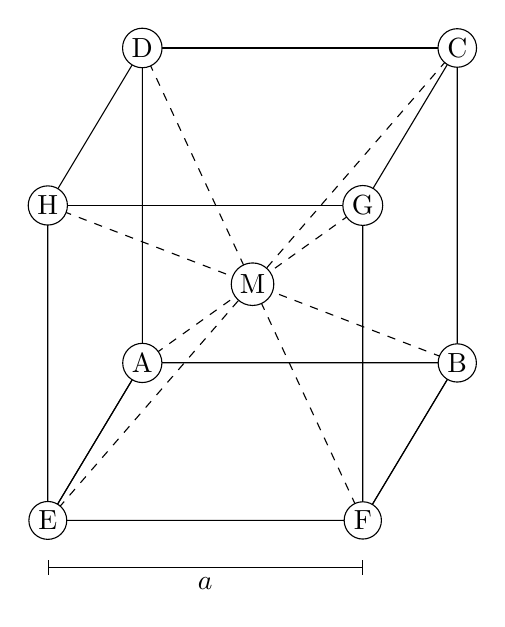
\begin{tikzpicture}[scale=2, z={(-3mm, -5mm)}]
		\coordinate (a) at (0, 0, 0);
		\coordinate (b) at (2, 0, 0);
		\coordinate (c) at (2, 2, 0);
		\coordinate (d) at (0, 2, 0);
		\coordinate (e) at (0, 0, 2);
		\coordinate (f) at (2, 0, 2);
		\coordinate (g) at (2, 2, 2);
		\coordinate (h) at (0, 2, 2);
		\coordinate (m) at (1, 1, 1);

		\draw (a) -- (b) -- (c) -- (d) -- (a);
		\draw (e) -- (f) -- (g) -- (h) -- (e);
		\draw (a) -- (d) -- (h) -- (e) -- (a);
		\draw (b) -- (c) -- (g) -- (f) -- (b);
		\draw (a) -- (b) -- (f) -- (e) -- (a);

		\draw[dashed] (a) -- (m);
		\draw[dashed] (b) -- (m);
		\draw[dashed] (c) -- (m);
		\draw[dashed] (d) -- (m);
		\draw[dashed] (e) -- (m);
		\draw[dashed] (f) -- (m);
		\draw[dashed] (g) -- (m);
		\draw[dashed] (h) -- (m);

		\node[draw, circle, fill=white, inner sep=.5mm] at (a) {A};
		\node[draw, circle, fill=white, inner sep=.5mm] at (b) {B};
		\node[draw, circle, fill=white, inner sep=.5mm] at (c) {C};
		\node[draw, circle, fill=white, inner sep=.5mm] at (d) {D};
		\node[draw, circle, fill=white, inner sep=.5mm] at (e) {E};
		\node[draw, circle, fill=white, inner sep=.5mm] at (f) {F};
		\node[draw, circle, fill=white, inner sep=.5mm] at (g) {G};
		\node[draw, circle, fill=white, inner sep=.5mm] at (h) {H};
		\node[draw, circle, fill=white, inner sep=.5mm] at (m) {M};

		\draw[|-|] (0, -.3, 2) -- ++(2, 0, 0) node[below, midway] {$a$};
	\end{tikzpicture}
	\caption{%
		bcc Zelle. Die Punkte A bis H sind die Eckpunkte, M ist der
		Mittelpunkt.
	}
	\label{fig:bcc}
\end{figure}

\subsection{Basisvektoren des Bravaisgitters}

Es handelt sich hier um einen Würfel mit Kantenlänge $a$, also sind die
Basisvektoren skalierte Versionen der kanonischen Basisvektoren des $\R^3$:
\[
	\vec t_i = a \ev_i
\]

\subsection{Volumina der Zellen}

Die konventionelle Zelle ist die, aus der man den ganzen Kristall durch
Translation aufbauen kann. Dies sollte dann das Parallelepiped sein, das von
den $\vec t_i$ aufgespannt wird. Da diese orthogonal sind und einen Würfel
aufspannen, ist das Volumen $V_\text{konv.} = a^3$.

Die Einheitszelle ist die, bei der nur an den Eckpunkten Atome sitzen. Dies ist
die quadratische Pyramide ABCDM aus Abbildung \ref{fig:bcc}. Das Volumen ist
ein Sechstel des ganzen Würfels, also:
\[
	V_\text{Einh.} = \frac{a^3}6
\]

\subsection{Gitterkonstante bestimmen}

Innerhalb einer konventionellen Zelle sind von den Eckatomen jeweils nur ein
Achtel, allerdings gibt es acht von ihnen. Und das mittlere Atom ist komplett
drin. Also sind pro Einheitszelle gerade zwei volle Atome enthalten. Die
Atomdichte $\nu$ ist also:
\[
	\nu = \frac{2}{a^3}
\]

Mit einer Dichte von $\rho = \SI{10.28}{\gram\per\centi\meter\cubed}$ und einer
Molaren Masse von $\SI{95.9}{\gram\per\mol}$ sind dies
\[
	\nu
	= \SI{107.2}{\milli\mol\per\centi\meter\cubed}
	= \SI{6.455e22}{\per\centi\meter\cubed}
\]

Somit erhalte ich für $a$:
\[
	a = \SI{3.141e-10}{\meter}
\]

Die Gitterkonstante ist also im Bereich einiger Atomradii, was anschaulich gut
passt.

\subsection{Welches Bravaisgitter?}

Das gesamte Gitter, wenn man ignoriert, dass es von zwei verschiedenen Ionen
besetzt ist, ist einfach nur kubisch.

Die Gitter von Chlor und Natrium einzeln sind kubisch flächenzentriert.

\subsection{Vektoren einzeichnen}

Die Vektoren $\vec t_n$ sind in Abbildung \ref{fig:bravaisgitter}, sowie die
Vektoren $\vec d_n$ in Abbildung \ref{fig:einheitszelle}. Dabei bin ich davon
ausgegangen, dass das interessantere Gitter der einzelnen Ionen gemeint ist.
Das kubische Gitter des Gesamtkristalls hat sowohl als Bravaisgitter, als auch
als konventionelle Zelle die gestreckten, kanonischen Basisvektoren des $\R^3$.

\begin{figure}[h]
	\centering
	\begin{tikzpicture}[scale=3, z={(-3mm, -5mm)}]

		\foreach \x in {0, ..., 1}
		\foreach \y in {0, ..., 2}
		\foreach \z in {0, ..., 2}
		\draw (\x, \y, \z) -- ++(1, 0, 0);

		\foreach \x in {0, ..., 2}
		\foreach \y in {0, ..., 1}
		\foreach \z in {0, ..., 2}
		\draw (\x, \y, \z) -- ++(0, 1, 0);

		\foreach \x in {0, ..., 2}
		\foreach \y in {0, ..., 2}
		\foreach \z in {0, ..., 1}
		\draw (\x, \y, \z) -- ++(0, 0, 1);

		\node[fill=white, draw, circle] (n1) at (0, 0, 0) {Na};
		\node[fill=white, draw, circle] (n2) at (2, 0, 0) {Na};
		\node[fill=white, draw, circle] (n3) at (2, 2, 0) {Na};
		\node[fill=white, draw, circle] (n4) at (0, 2, 0) {Na};
		\node[fill=white, draw, circle] (n4) at (1, 1, 0) {Na};
		\node[fill=white, draw, circle] (n1) at (1, 0, 1) {Na};
		\node[fill=white, draw, circle] (n2) at (1, 2, 1) {Na};
		\node[fill=white, draw, circle] (n3) at (2, 1, 1) {Na};
		\node[fill=white, draw, circle] (n4) at (0, 1, 1) {Na};
		\node[fill=white, draw, circle] (n5) at (0, 0, 2) {Na};
		\node[fill=white, draw, circle] (n6) at (2, 0, 2) {Na};
		\node[fill=white, draw, circle] (n7) at (2, 2, 2) {Na};
		\node[fill=white, draw, circle] (n8) at (0, 2, 2) {Na};
		\node[fill=white, draw, circle] (n4) at (1, 1, 2) {Na};

		\draw[->, very thick, color=darkgreen] (0, 0, 2) -- ++(2, 0, 0) node[midway, above, sloped] {$\vec t_1$};
		\draw[->, very thick, color=darkgreen] (0, 0, 2) -- ++(0, 2, 0) node[midway, above, sloped] {$\vec t_3$};
		\draw[->, very thick, color=darkgreen] (0, 0, 2) -- ++(0, 0, -2) node[midway, above, sloped] {$\vec t_2$};

	\end{tikzpicture}
	\caption{%
		Das kubisch flächenzentrierte Gitter des Natriums. Eingezeichnet sind
		die Vektoren, die das Bravaisgitter aufspannen.
	}
	\label{fig:bravaisgitter}
\end{figure}

\begin{figure}[h]
	\centering
	\begin{tikzpicture}[scale=3, z={(-3mm, -5mm)}]

		\foreach \x in {0, ..., 1}
		\foreach \y in {0, ..., 2}
		\foreach \z in {0, ..., 2}
		\draw (\x, \y, \z) -- ++(1, 0, 0);

		\foreach \x in {0, ..., 2}
		\foreach \y in {0, ..., 1}
		\foreach \z in {0, ..., 2}
		\draw (\x, \y, \z) -- ++(0, 1, 0);

		\foreach \x in {0, ..., 2}
		\foreach \y in {0, ..., 2}
		\foreach \z in {0, ..., 1}
		\draw (\x, \y, \z) -- ++(0, 0, 1);

		\node[fill=white, draw, circle] (n1) at (0, 0, 0) {Na};
		\node[fill=white, draw, circle] (n2) at (2, 0, 0) {Na};
		\node[fill=white, draw, circle] (n3) at (2, 2, 0) {Na};
		\node[fill=white, draw, circle] (n4) at (0, 2, 0) {Na};
		\node[fill=white, draw, circle] (n4) at (1, 1, 0) {Na};
		\node[fill=white, draw, circle] (n1) at (1, 0, 1) {Na};
		\node[fill=white, draw, circle] (n2) at (1, 2, 1) {Na};
		\node[fill=white, draw, circle] (n3) at (2, 1, 1) {Na};
		\node[fill=white, draw, circle] (n4) at (0, 1, 1) {Na};
		\node[fill=white, draw, circle] (n5) at (0, 0, 2) {Na};
		\node[fill=white, draw, circle] (n6) at (2, 0, 2) {Na};
		\node[fill=white, draw, circle] (n7) at (2, 2, 2) {Na};
		\node[fill=white, draw, circle] (n8) at (0, 2, 2) {Na};
		\node[fill=white, draw, circle] (n4) at (1, 1, 2) {Na};

		\draw[->, very thick, color=darkblue] (0, 0, 2) -- ++(1, 0, -1) node[midway, above, sloped] {$\vec d_1$};
		\draw[->, very thick, color=darkblue] (0, 0, 2) -- ++(0, 1, -1) node[midway, above, sloped] {$\vec d_3$};
		\draw[->, very thick, color=darkblue] (0, 0, 2) -- ++(0, 0, -2) node[midway, above, sloped] {$\vec d_2$};

	\end{tikzpicture}
	\caption{%
		Das kubisch flächenzentrierte Gitter des Natriums. Eingezeichnet sind
		die Vektoren, die die Einheitszelle aufspannen.
	}
	\label{fig:einheitszelle}
\end{figure}

\subsection{Gitterkonstante von Natriumchlorid}

In einer kubischen Zelle, die die Kantenlänge $a/2$ hat, ist jeweils ein halbes
Chlor- und ein halbes Natriumion enthalten. In einer ganzen konventionellen
Zelle sind also acht mal so viele, also vier Ionenpaare enthalten.

Die Dichte ist $\varrho = \SI{2.17}{\gram\per\centi\meter\cubed}$. Die Masse
pro Ionenpaar ist $m = \SI{9.70e-23}{\gram}$. Das eingenommene Volumen pro
Ionenpaar ist $m/\varrho$, die Größe der Zellen ist $4m/\varrho$. Die
Kubikwurzel daraus ist dann die Gitterkonstante $a = \SI{5.63e-10}\meter$.

%%%%%%%%%%%%%%%%%%%%%%%%%%%%%%%%%%%%%%%%%%%%%%%%%%%%%%%%%%%%%%%%%%%%%%%%%%%%%%%
%                              Reziprokes Gitter                              %
%%%%%%%%%%%%%%%%%%%%%%%%%%%%%%%%%%%%%%%%%%%%%%%%%%%%%%%%%%%%%%%%%%%%%%%%%%%%%%%

\section{Reziprokes Gitter}
\label 3

\subsection{Bravaisvektoren}

In der Ebene brauche ich zwei Vektoren. Ich benutze dazu (in Polarkoordinaten):
\[
	\vec t_1 = a \angle \SI{-30}\degree
	\eqnsep
	\vec t_2 = a \angle \SI{90}\degree
\]

In kartesischen Koordinaten ist dies:
\[
	\vec t_1 = a
	\begin{pmatrix}
		\cos\del{\SI{30}\degree} \\
		- \sin\del{\SI{30}\degree}
	\end{pmatrix}
	= a
	\begin{pmatrix}
		\sqrt{3}/2 \\
		- \num{.5}
	\end{pmatrix}
	\eqnsep
	\vec t_2 = a
	\begin{pmatrix}
		0 \\ 1
	\end{pmatrix}
\]

Diese sind in Abbildung \ref{fig:3a} eingezeichnet.

\begin{figure}[h]
	\centering
	\begin{tikzpicture}[scale=2]
		\draw (0, 0)
		-- ++(0, 1)
		-- ++(.866, .5)
		-- ++(.866, -.5)
		-- ++(0, -1)
		-- ++(-.866, -.5)
		-- ++(-.866, .5);

		\draw (0, 0)
		-- ++(.866, -.5)
		-- ++(0, -1)
		-- ++(-.866, -.5)
		-- ++(-.866, .5)
		-- ++(0, 1)
		-- ++(.866, .5)
		-- ++(.866, -.5)
		-- ++(0, -1)
		-- ++(-.866, -.5)
		-- ++(-.866, .5);

		\draw (0, 0) ++(-150:1) ++(150:1)
		-- ++(0, 1)
		-- ++(.866, .5)
		-- ++(.866, -.5)
		-- ++(0, -1)
		-- ++(-.866, -.5)
		-- ++(-.866, .5);

		\draw[very thick, red, ->] (0, 0) -- ++(.866, -.5) node[midway, sloped, below] {$\vec t_1$};
		\draw[very thick, red, ->] (0, 0) -- ++(0, 1) node[midway, sloped, above] {$\vec t_2$};

		\draw[very thick, darkgreen, ->] (0, -2) -- ++(150:3);
		\draw[very thick, darkgreen, ->] (0, -2) -- ++(60:3.464);
	\end{tikzpicture}
	\caption{%
		Bravaisvektoren für Graphen in rot. In Grün die Basisvektoren der
		konventionellen Zelle.
	}
	\label{fig:3a}
\end{figure}

\subsection{Reziprokes Gitter}

Das reziproke Gitter $\vec g_i$ hat als definierende Eigenschaft:
\[
	\inner{\vec t_i}{\vec g_j} = 2 \piup \delta_{ij}
\]

Also suche ich einen Vektor $\vec g_1$, der auf $\vec t_2$ senkrecht steht, und
auf $\vec t_1$ projiziert die Länge $2\piup$ hat. Dieser muss proportional zu
$\ev_x$ sein. Durch Raten erhalte ich:
\[
	\vec g_1 = \frac{2\piup}a \begin{pmatrix}
		2 / \sqrt 3 \\ 0
	\end{pmatrix}
\]

Diesen Vektor drehe ich um \SI{-120}{\degree}, so dass dieser senkrecht auf $\vec t_1$ steht und erhalte damit dann $\vec g_2$. Die Rotationsmatrix ist:
\[
	\tens R_{\SI{-120}\degree} =
	\begin{pmatrix}
		- \half & - \frac{\sqrt 3}2 \\
		- \frac{\sqrt 3}2 & \half
	\end{pmatrix}
\]

Dadurch wird der Vektor:
\[
	\vec g_2
	= \frac{2\piup}a
	\begin{pmatrix}
		- \frac1{\sqrt{3}} \\ - 1
	\end{pmatrix}
\]

Dieser Vektor ist senkrecht auf $\vec t_1$ und hat die Länge $2\piup$, wenn auf $\vec t_2$ projiziert.

Beim normalen Gitter hatte ich auch noch die Differenz der beiden Vektoren
gebraucht, um das ganze Sechseck zu bekommen. Wahrscheinlich brauche ich dann
auch hier die Differenz, allerdings an nur einigen Stellen, die Gitterpunkte im
reziproken Gitter zu erhalten. Das reziproke Gitter sollte ebenfalls die
Wabenstruktur haben, allerdings so verkippt, dass es horizontale
Verbindungslinien gibt.

\subsection{Erste Brilloinzone}

\fehlt

\subsection{Millerindizes}

\fehlt

%%%%%%%%%%%%%%%%%%%%%%%%%%%%%%%%%%%%%%%%%%%%%%%%%%%%%%%%%%%%%%%%%%%%%%%%%%%%%%%
%                     Bragg-Beugung und Röntgenstrahlung                     %
%%%%%%%%%%%%%%%%%%%%%%%%%%%%%%%%%%%%%%%%%%%%%%%%%%%%%%%%%%%%%%%%%%%%%%%%%%%%%%%

\section{Bragg-Beugung und Röntgenstrahlung}
\label 4

\fehlt

%%%%%%%%%%%%%%%%%%%%%%%%%%%%%%%%%%%%%%%%%%%%%%%%%%%%%%%%%%%%%%%%%%%%%%%%%%%%%%%
%                                    Ende                                     %
%%%%%%%%%%%%%%%%%%%%%%%%%%%%%%%%%%%%%%%%%%%%%%%%%%%%%%%%%%%%%%%%%%%%%%%%%%%%%%%

\IfFileExists{\bibliographyfile}{
	\bibliography{\bibliographyfile}
}{}

\end{document}

% vim: spell spelllang=de
